\section{The number of projects}

In the vast majority of cases a programmer works on one project per day according to the data \ref{fig:projects_per_day}. Cases with 5 or more projects were not recorded. Situations were no projects were recorded during the day (i.e. a user in VS Code works outside the named workspace) remain very scarce.

\begin{figure}[htbp]
  \centering
  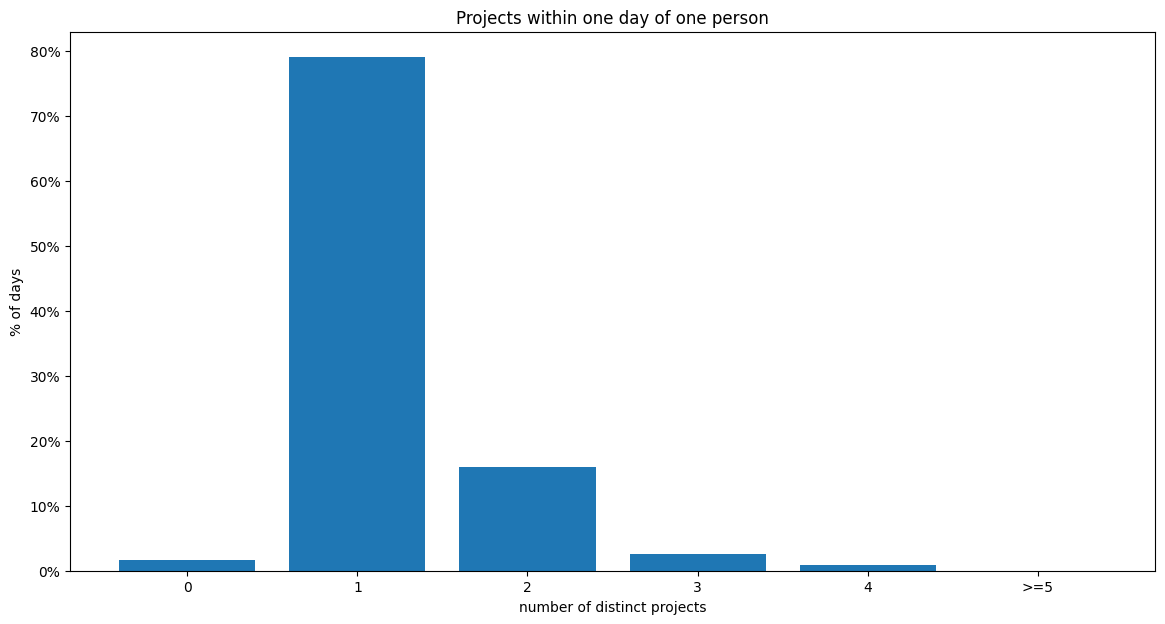
\includegraphics[scale=0.5]{chapters/results/graphics/projects-day.png}
  \caption{Number of projects within one day of a programmer}
  \label{fig:projects_per_day}
\end{figure}

A similar picture is observed even when considering all the projects of one person within the time frame of my research \ref{fig:projects_per_person}. Cases with 6 or more recorded projects per person were uncommon and most oscillated between 1 and 3.

\begin{figure}[htbp]
  \centering
  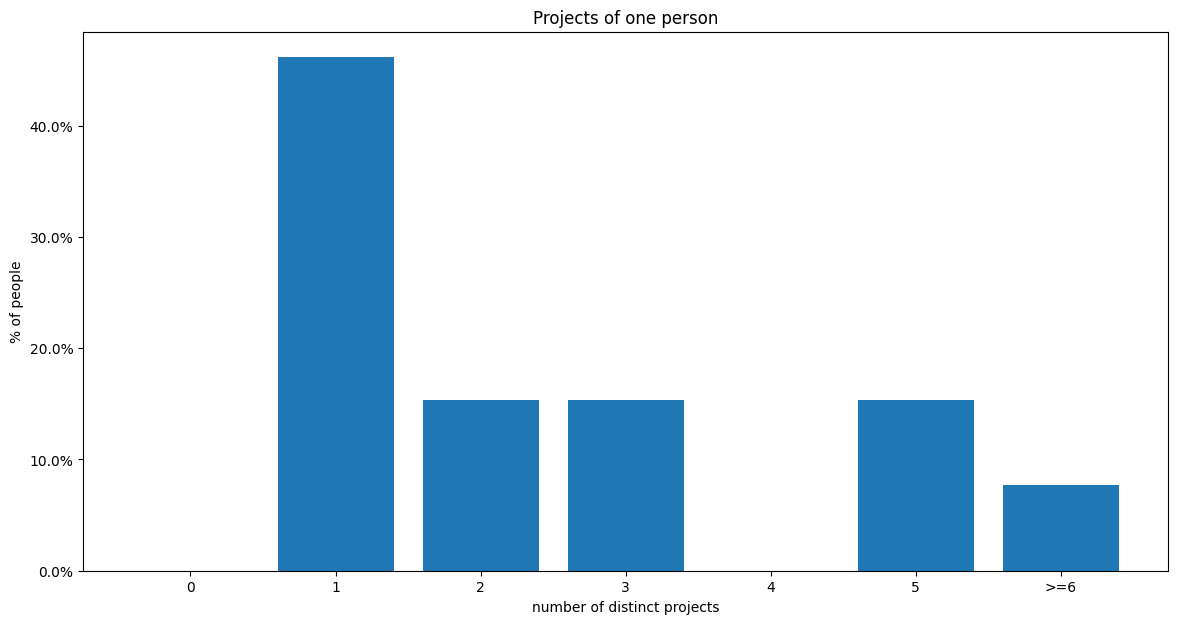
\includegraphics[scale=0.5]{chapters/results/graphics/projects-one-person.png}
  \caption{Number of programmer's projects}
  \label{fig:projects_per_person}
\end{figure}

It turns out that according to the data it is also uncommon to switch projects during the working day \ref{fig:projects_switching_per_day}. During the staggering most of the days developers did not switch the project even once.

\begin{figure}[htbp]
  \centering
  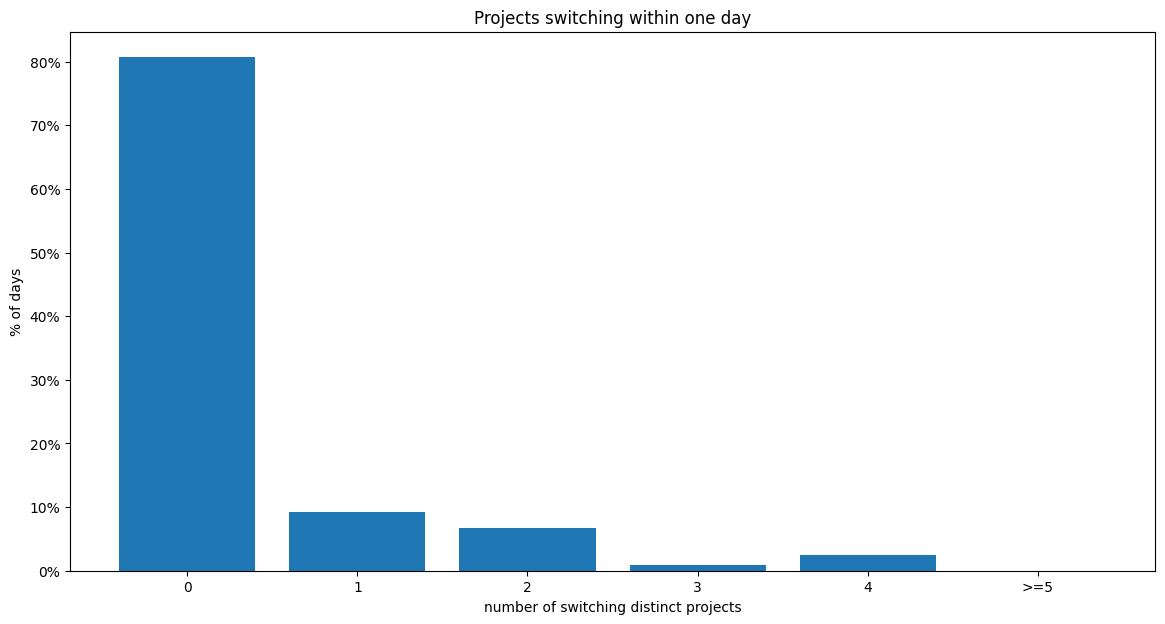
\includegraphics[scale=0.5]{chapters/results/graphics/projects-switching-day.png}
  \caption{Number of projects switching within one day of a programmer}
  \label{fig:projects_switching_per_day}
\end{figure}
